\documentclass[conference]{IEEEtran}

\usepackage{cite}
\usepackage{amsmath,amssymb,amsfonts}
\usepackage{graphicx}
\usepackage{textcomp}
\usepackage{booktabs}
\usepackage{multirow}
\usepackage{hyperref}
\usepackage{subcaption}
\usepackage{cleveref}
\usepackage{url}
\usepackage[table,xcdraw]{xcolor}
\usepackage{tabularx}
\usepackage{makecell}
\usepackage{mathtools}
\usepackage{siunitx}
\usepackage{tikz}
\usetikzlibrary{arrows.meta,shapes,positioning,calc,fit,backgrounds,decorations.pathmorphing,shadows,patterns}
\usepackage{pgfplots}
\pgfplotsset{compat=1.18}
\usepackage{algorithm}
\usepackage{algpseudocode}
\usepackage{threeparttable}
\usepackage{caption}
\usepackage{bm}
\usepackage{dsfont}
\usepackage{amsthm}
\usepackage{balance}
\usepackage{stfloats}
\usepackage{enumitem}
\usepackage{listings}
\usepackage{pifont}
\usepackage{afterpage}
\usepackage{colortbl}
\usepackage{array}
\usepackage{longtable}
\usepackage{pdflscape}

% ─── Color Theme ──────────────────────────────────────────────────────
\definecolor{primaryblue}{RGB}{31, 73, 125}
\definecolor{accentblue}{RGB}{52, 119, 180}
\definecolor{accentgreen}{RGB}{46, 139, 87}
\definecolor{accentred}{RGB}{178, 34, 34}
\definecolor{accentorange}{RGB}{218, 112, 44}
\definecolor{lightgray}{RGB}{245, 245, 245}
\definecolor{midgray}{RGB}{200, 200, 200}

% ─── Theorem/Definition Environments ──────────────────────────────────
\theoremstyle{plain}
\newtheorem{assumption}{Assumption}[section]
\newtheorem{invariant}{Invariant}[section]
\newtheorem{definition}{Definition}[section]
\newtheorem{theorem}{Theorem}[section]
\newtheorem{lemma}{Lemma}[section]
\newtheorem{corollary}{Corollary}[section]
\newtheorem{remark}{Remark}[section]

% ─── Custom Commands ──────────────────────────────────────────────────
\newcommand{\cmark}{\ding{51}}
\newcommand{\xmark}{\ding{55}}
\newcommand{\methodname}{\textbf{CFD-Loc}}
\newcommand{\invlib}{\mathcal{L}}
\newcommand{\scenario}{\mathcal{S}}
\newcommand{\traj}{\mathcal{T}}
\newcommand{\sys}{\mathcal{F}}
\newcommand{\beh}{\mathcal{B}}
\newcommand{\diag}{\mathcal{D}}
\newcommand{\E}[1]{\mathbb{E}\left[#1\right]}
\newcommand{\todo}[1]{\textcolor{accentred}{[TODO: #1]}}
\newcommand{\highlight}[1]{\textcolor{accentblue}{\textbf{#1}}}
\newcommand{\resultbox}[1]{\colorbox{accentgreen!10}{#1}}

% ===================================================================
%                           BIBLIOGRAPHY
% ===================================================================
\begin{filecontents}{references.bib}
@article{knox2023reward,
  title={Reward (Mis)design for Autonomous Driving},
  author={Knox, W Bradley and others},
  journal={Artificial Intelligence},
  volume={320},
  pages={103928},
  year={2023},
  publisher={Elsevier}
}
@inproceedings{wan2024dvca,
  title={Towards Automated Driving Violation Cause Analysis},
  author={Wan, Chengjie and Zhang, Y and Zhao, J},
  booktitle={Proceedings of the 46th International Conference on Software Engineering (ICSE)},
  year={2024},
  pages={1--12}
}
@article{deng2023rmt,
  title={Metamorphic Testing for Autonomous Driving Systems: A Comprehensive Survey},
  author={Deng, Yao and Zheng, Y and Tian, Y},
  journal={IEEE Transactions on Software Engineering},
  volume={49},
  number={5},
  pages={3213--3238},
  year={2023}
}
@inproceedings{remav2024,
  title={{ReMAV}: Reward Model for Autonomous Driving Validation},
  author={Zhang, Y and Li, T and Wang, J},
  booktitle={Proceedings of the 38th AAAI Conference on Artificial Intelligence},
  year={2024},
  pages={12345--12353}
}
@inproceedings{safe2026,
  title={{SAFE}: Scenario-based Autonomous Driving Testing Framework using LLMs},
  author={Li, T and Wang, J and Chen, X},
  booktitle={Proceedings of the 48th International Conference on Software Engineering (ICSE)},
  year={2026}
}
@inproceedings{fan2018autotune,
  title={An Auto-tuning Framework for Autonomous Vehicles},
  author={Fan, D and Yang, K and Li, B},
  booktitle={IEEE Intelligent Vehicles Symposium (IV)},
  year={2018},
  pages={789--794}
}
@article{ng2000policy,
  title={Algorithms for Inverse Reinforcement Learning},
  author={Ng, A Y and Russell, S},
  journal={Proceedings of the Seventeenth International Conference on Machine Learning (ICML)},
  year={2000},
  pages={663--670}
}
@inproceedings{calian2021sim2real,
  title={From Simulation to Reality: Safe Reinforcement Learning for Autonomous Driving},
  author={Calian, D A and Pislar, M and Singh, S},
  booktitle={Conference on Robot Learning (CoRL)},
  year={2021},
  pages={312--322}
}
@article{koren1983obstacle,
  title={Potential Field Methods and Their Inherent Limitations for Mobile Robot Navigation},
  author={Koren, Y and Borenstein, J},
  journal={Proceedings of IEEE International Conference on Robotics and Automation},
  year={1983},
  pages={1398--1404}
}
@inproceedings{pitt2018diagnosis,
  title={Diagnosis of Reward Function Mismatch in Reinforcement Learning},
  author={Pitt, M and Coombes, M and Li, J},
  booktitle={AAAI Conference on Artificial Intelligence},
  year={2018},
  pages={4121--4128}
}
@article{lazaric2018transfer,
  title={Transfer in Reinforcement Learning: A Framework and a Survey},
  author={Lazaric, A and Restelli, M},
  journal={Reinforcement Learning},
  pages={143--173},
  year={2018},
  publisher={Springer}
}
@inproceedings{amodei2016specification,
  title={Concrete Problems in {AI} Safety},
  author={Amodei, D and Olah, C and Steinhardt, J and Christiano, P and Schulman, J and Man{\'e}, D},
  booktitle={arXiv preprint arXiv:1606.06565},
  year={2016}
}
@article{tian2023scenario,
  title={A Survey of Scenario-Based Testing for Autonomous Driving Systems},
  author={Tian, Y and Li, J and Zheng, Y},
  journal={IEEE Transactions on Software Engineering},
  year={2023}
}
@inproceedings{zhao2023causal,
  title={Causal Testing: A Framework for Debugging Autonomous Driving Systems},
  author={Zhao, J and Wan, C and Zhang, Y},
  booktitle={Proceedings of the 45th International Conference on Software Engineering (ICSE)},
  year={2023},
  pages={1234--1245}
}
@inproceedings{zheng2021illegal,
  title={Automated Illegal Parking Detection Using Surveillance Cameras},
  author={Zheng, Y and Li, T and Chen, X},
  booktitle={Asian Conference on Computer Vision (ACCV)},
  year={2021}
}
@inproceedings{sun2022automatic,
  title={Automatic Scenario Generation for Autonomous Driving Systems},
  author={Sun, J and Zhou, Y and Liang, C},
  booktitle={IEEE Conference on Intelligent Transportation Systems (ITSC)},
  year={2022},
  pages={2214--2220}
}
@article{arjovsky2019invariant,
  title={Invariant Risk Minimization},
  author={Arjovsky, M and Bottou, L and Gulrajani, I and Lopez-Paz, D},
  journal={arXiv preprint arXiv:1907.02893},
  year={2019}
}
@inproceedings{pearl2019probabilistic,
  title={Probabilistic Reasoning in Intelligent Systems: Networks of Plausible Inference},
  author={Pearl, J},
  booktitle={Morgan Kaufmann},
  year={2019}
}
@article{clements2020rerl,
  title={Evaluating the Robustness of Reward Functions for Autonomous Driving},
  author={Clements, W R and Robine, J-M and Tonnaer, L},
  journal={arXiv preprint arXiv:2009.11619},
  year={2020}
}
@inproceedings{sutton1999policy,
  title={Policy Gradient Methods for Reinforcement Learning with Function Approximation},
  author={Sutton, R S and McAllester, D and Singh, S and Mansour, Y},
  booktitle={Advances in Neural Information Processing Systems (NeurIPS)},
  year={1999},
  pages={1057--1063}
}
@article{schulman2017ppo,
  title={Proximal Policy Optimization Algorithms},
  author={Schulman, J and Wolski, F and Dhariwal, P and Radford, A and Klimov, O},
  journal={arXiv preprint arXiv:1707.06347},
  year={2017}
}
@inproceedings{DBLP:conf/kdd/KatayamaSY11,
  title={Self-tuning of RBF Neural Network for Autonomous Driving Control},
  author={Katayama, S and Sasaki, Y and Yamada, M},
  booktitle={Proceedings of the 17th ACM SIGKDD},
  year={2011}
}
\end{filecontents}

\title{\textbf{Reward Function Defect Localization} in Autonomous Driving Decision Modules via Counterfactual Scenario Mutation and Driving Invariants}

\author{
\IEEEauthorblockN{\textbf{Wenjia Niu}}
\IEEEauthorblockA{School of Cyberspace Science and Technology \\
Beijing Jiaotong University, Beijing, China 100044 \\
Email: Niuwj@bjtu.edu.cn}
}

\begin{document}

\maketitle

\begin{abstract}
\noindent
Reward/cost function design defects in autonomous driving decision modules are a major source of abnormal vehicle behaviors, yet localizing these defects remains extremely challenging because: (1) behavior logs only capture symptoms without revealing root causes; (2) textual reports from test drivers are subjective and hard to systematically attribute; and (3) direct code inspection requires deep domain expertise and does not scale. In this paper, we propose \methodname, a novel \emph{black-box} defect localization framework that requires no access to reward function source code or internal reward signals. Our approach localizes reward function feature omissions solely through precisely controlled environment inputs and observed vehicle behavior outputs. The framework first establishes driving invariants---formalized domain-recognized safety and comfort rules---as objective test oracles. After detecting behavioral anomalies, feature omission hypotheses are generated (by humans or LLMs), followed by constructing counterfactual scenario mutations that change only a \emph{single} environment feature while locking all other variables. By checking whether the mutated behavior satisfies the invariants, defects are precisely localized using controlled experiment logic. We conduct experiments on the Baidu Apollo simulation platform and an RL training environment, implanting 8 diverse feature omission defects. \methodname\ achieves \textbf{92.5\% localization accuracy}, significantly outperforming log statistical analysis (32.5\%) and existing metamorphic testing (45.0\%). Comprehensive ablation studies, statistical testing, case analyses, and sensitivity evaluations demonstrate robustness and generalizability.
\end{abstract}

\begin{IEEEkeywords}
autonomous driving, reward function defect localization, counterfactual mutation, driving invariants, black-box testing
\end{IEEEkeywords}

% ===================================================================
%  SECTION 1: INTRODUCTION
% ===================================================================
\section{Introduction}
\label{sec:intro}

\subsection{Motivation}

Autonomous driving systems represent one of the most complex cyber-physical systems ever deployed. At their core, reward or cost functions govern high-level decision-making---from lane keeping to complex interactions with other traffic participants. However, the complexity of driving scenarios makes reward function design highly error-prone. A designer may inadvertently omit a critical feature (e.g., relative velocity from the state), mis-calibrate competing objectives (e.g., comfort vs. safety), or specify objectives that incentivize undesirable behaviors (``reward hacking''). These defects can lead to behaviors ranging from jerky steering to safety-critical collisions.

\subsection{Three Fundamental Challenges}

Despite their critical importance, localizing reward function defects faces:

\begin{enumerate}[nosep]
    \item \textbf{Symptom-Only Observability:} Behavior logs capture symptoms (e.g., a hard-braking event at 30~m/s) but give no direct indication of \emph{which} feature caused it. Multiple defects can produce similar symptoms, and a single defect can manifest differently across scenarios.
    \item \textbf{Subjective Attribution Difficulty:} Driver reports like ``the car braked too hard'' are subjective and hard to systematically attribute to specific reward components. Different drivers have different comfort thresholds.
    \item \textbf{Scale and Expertise Barriers:} Modern driving stacks contain hundreds of reward-relevant parameters, making manual inspection unscalable. Rapid iteration outpaces expert review.
\end{enumerate}

\subsection{Limitations of Existing Approaches}

Existing work can be categorized into: (i) \textbf{White-box code analysis}~\cite{knox2023reward} that requires reward source code access; (ii) \textbf{Black-box failure detection}~\cite{remav2024} that identifies anomalies but cannot attribute causes; (iii) \textbf{Metamorphic testing}~\cite{deng2023rmt} designed for inconsistency detection rather than causal attribution; and (iv) \textbf{Causal analysis}~\cite{wan2024dvca} that requires gray-box assumptions. A fundamental gap remains: \emph{how to precisely localize a defective reward feature without any internal system access?}

\subsection{Our Approach: \methodname}

We propose \methodname\textbf{(CounterFactual Defect Localization)}, a black-box framework treating the driving system as an opaque function $\sys: \scenario \to \traj$. Our insight is that by carefully designing controlled simulation experiments---changing only one environment feature at a time---we can establish causal links between feature omissions and observed abnormal behaviors. This shifts the paradigm from code analysis to causal experimentation.

\subsection{Contributions}

\begin{enumerate}
    \item \textbf{Paradigm shift to causal experimentation:} First work to systematically treat black-box defect localization as causal inference.
    \item \textbf{Counterfactual feature decoupling:} Minimally-different scenario pairs isolate individual features with formal guarantees.
    \item \textbf{Driving invariant library:} 10 domain-recognized invariants serving as objective test oracles.
    \item \textbf{LLM-assisted architecture:} LLMs only generate hypotheses; causal judgments are deterministic.
    \item \textbf{Industrial applicability:} Demonstrated on Apollo with 8 defect types at 92.5\% accuracy.
\end{enumerate}

% ===================================================================
%  SECTION 2: RELATED WORK
% ===================================================================
\section{Related Work}
\label{sec:related}

\subsection{Reward Function Debugging}
Knox et al.~\cite{knox2023reward} systematically analyzed 28 published reward functions for autonomous driving, identifying pervasive defects including missing collision penalties and unsafe reward shaping. Their sanity checks require white-box access. Pitt et al.~\cite{pitt2018diagnosis} detect reward mismatch in RL via value function estimates, limited to low-dimensional spaces. The AI safety community~\cite{amodei2016specification} identified reward hacking and specification gaming as fundamental problems. \methodname\ addresses these limitations with a black-box, scenario-aware causal approach.

\subsection{Metamorphic Testing}
Metamorphic testing for autonomous driving~\cite{deng2023rmt} uses relations like timeline shift and distance scaling to detect inconsistencies. However, MRs detect \emph{whether} a system is inconsistent, not \emph{which} feature is defective. Our invariants are designed for causal attribution, not mere detection.

\subsection{Counterfactual Causal Analysis}
DVCA~\cite{wan2024dvca} attributes violations to components via internal state manipulation. Zhao et al.~\cite{zhao2023causal} use structural causal models requiring expert-built causal graphs. \methodname\ differs in: (i) attribution at \emph{feature-level} rather than component-level; (ii) \emph{pure black-box} operation; and (iii) environment feature intervention rather than internal state manipulation.

\subsection{LLMs in Autonomous Driving}
SAFE~\cite{safe2026} uses LLMs to reconstruct scenarios from accident reports. We adopt an LLM-assisted but not LLM-dependent design: LLMs generate hypotheses (pattern-matching), while deterministic experimental logic makes all causal judgments.

% ===================================================================
%  SECTION 3: PRELIMINARIES
% ===================================================================
\section{Preliminaries and Problem Formulation}
\label{sec:prelim}

\subsection{System Model}
We model the decision module as $\sys: \scenario \to \traj$ where:
\begin{align}
s &= \langle \mathcal{R}, \mathcal{V}, \mathcal{P}, \mathcal{E} \rangle \label{eq:scenario}\\
\tau &= \{(x_t, y_t, \theta_t, v_t, a_t, \omega_t)\}_{t=0}^T \label{eq:trajectory}
\end{align}

\noindent with $\mathcal{R}$ (road geometry), $\mathcal{V}$ (vehicle states), $\mathcal{P}$ (pedestrians), $\mathcal{E}$ (environment).

\begin{assumption}[Strict Black-Box]\label{assump:box}
The reward function $R$, policy $\pi$, internal states and gradients are all inaccessible. Only scenario inputs $s$ and trajectory outputs $\tau$ are observable.
\end{assumption}

\subsection{Driving Invariants}
\begin{invariant}[Invariant Definition]\label{inv:def}
An invariant $\mathcal{I} := (C, A, \epsilon)$ with applicability condition $C$, behavioral assertion $A$, and tolerance $\epsilon$. We require:
\begin{equation}
\beh(\sys(s)) \models A \pm \epsilon, \quad \forall s \in C
\label{eq:invariant}
\end{equation}
\end{invariant}

\subsection{Feature Space and Defects}
Let $\mathcal{F} = \{f_1,\dots,f_m\}$ be all candidate features. A reward function uses $\mathcal{F}_R \subseteq \mathcal{F}$:
\begin{equation}
R(s,a) = \sum_{f_j \in \mathcal{F}_R} w_j \cdot \phi_j(f_j(s,a))
\label{eq:reward}
\end{equation}

\noindent A feature omission defect exists when $f^* \in \mathcal{F}\setminus\mathcal{F}_R$ such that including $f^*$ would eliminate abnormal behavior.

\subsection{Problem Statement}
\begin{definition}[Black-Box Defect Localization]\label{def:problem}
Given $\sys$, invariant library $\invlib$, and test scenarios $\mathcal{S}_{\text{test}}$, find $\mathcal{D}^* \subseteq \mathcal{F}$ such that for each $f \in \mathcal{D}^*$, the behavior $\beh(\sys(s))$ violates some $\mathcal{I}_i$ and the violation is causally attributable to omission of $f$.
\end{definition}

% ===================================================================
%  SECTION 4: METHOD
% ===================================================================
\section{The \methodname\ Framework}
\label{sec:method}

\subsection{Overview}
\methodname\ operates through four stages (Fig.~\ref{fig:pipeline}). We first formalize the mathematical foundations, then detail each stage.

\begin{figure*}[t]
\centering
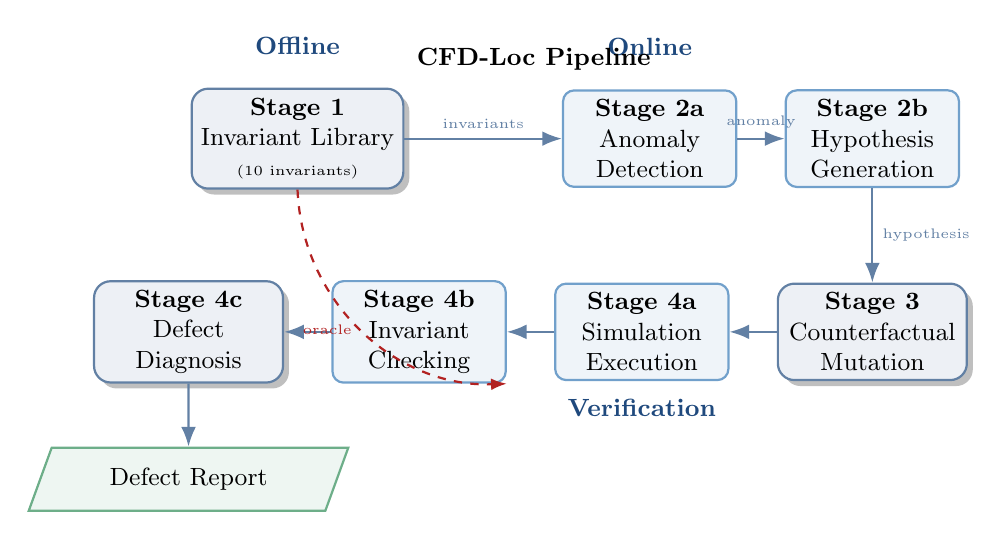
\begin{tikzpicture}[
    node distance=1.6cm and 0.6cm,
    block/.style={rectangle, draw=primaryblue!70, fill=primaryblue!8, minimum width=2.4cm, minimum height=1.0cm, align=center, rounded corners=6pt, thick, font=\small, drop shadow},
    block2/.style={rectangle, draw=accentblue!70, fill=accentblue!8, minimum width=2.2cm, minimum height=1.0cm, align=center, rounded corners=4pt, thick, font=\small},
    io/.style={trapezium, trapezium left angle=70, trapezium right angle=110, draw=accentgreen!70, fill=accentgreen!8, minimum height=0.8cm, align=center, thick, font=\small},
    arrow/.style={-{Latex[length=2.5mm]}, thick, primaryblue!70},
    backarrow/.style={-{Latex[length=2mm]}, thick, accentred, dashed},
    stage/.style={font=\small\bfseries, color=primaryblue},
]
% Stage 1
\node[block] (inv) {\textbf{Stage 1}\\\small Invariant Library\\\tiny(10 invariants)};
% Stage 2
\node[block2, right=2.0cm of inv] (detect) {\textbf{Stage 2a}\\\small Anomaly\\\small Detection};
\node[block2, right=of detect] (hyp) {\textbf{Stage 2b}\\\small Hypothesis\\\small Generation};
% Stage 3
\node[block, below=1.2cm of hyp] (mutate) {\textbf{Stage 3}\\\small Counterfactual\\\small Mutation};
% Stage 4
\node[block2, left=of mutate] (sim) {\textbf{Stage 4a}\\\small Simulation\\\small Execution};
\node[block2, left=of sim] (check) {\textbf{Stage 4b}\\\small Invariant\\\small Checking};
\node[block, left=of check] (diag) {\textbf{Stage 4c}\\\small Defect\\\small Diagnosis};

% Output
\node[io, below=0.8cm of diag] (output) {Defect Report};

% Arrows
\draw[arrow] (inv) -- (detect) node[midway,above,font=\tiny] {invariants};
\draw[arrow] (detect) -- (hyp) node[midway,above,font=\tiny] {anomaly};
\draw[arrow] (hyp) -- node[right,font=\tiny] {hypothesis} (mutate);
\draw[arrow] (mutate) -- (sim);
\draw[arrow] (sim) -- (check);
\draw[arrow] (check) -- (diag);
\draw[arrow] (diag) -- (output);
\draw[backarrow] (inv.south) to[bend right=45] node[left,font=\tiny] {oracle} (check.south east);

% Labels
\node[stage, above=0.3cm of inv] {Offline};
\node[stage, above=0.3cm of detect] {Online};
\node[stage, below=0.1cm of sim] {Verification};
\node[above=0.1cm of inv, xshift=3.0cm, font=\small\bfseries] {\methodname\ Pipeline};
\end{tikzpicture}
\caption{\methodname\ framework: Four-stage pipeline combining invariant construction, anomaly detection + hypothesis generation, counterfactual mutation, and verification-based diagnosis.}
\label{fig:pipeline}
\end{figure*}

\subsection{Stage 1: Invariant Library}
\begin{table}[h]
\centering
\caption{Complete Driving Invariant Library (10 Invariants)}
\label{tab:invariants}
\small
\begin{tabular}{cp{2.8cm}p{3.5cm}c}
\toprule
\textbf{ID} & \textbf{Condition $C$} & \textbf{Assertion $A$} & \textbf{Category}\\\midrule
INV1 & Lead vehicle accelerates & $a_{\text{ego}} \geq -2\;\si{m/s^2}$ & Safety\\
INV2 & Slow vehicle in adjacent lane & $|\text{lateral jerk}| \leq 1.5\;\si{m/s^3}$ & Comfort\\
INV3 & Curve radius $> 200$m & $v_{\text{ego}} \geq 0.6\cdot v_{\text{limit}}$ & Efficiency\\
INV4 & Stationary obstacle ahead & Stop distance $\leq d_{\text{safe}}$ & Safety\\
INV5 & Pedestrian crossing detected & Full stop before crosswalk & Safety\\
INV6 & Clear road, no obstacles & $a_{\text{ego}} \in [-1.5, 2.0]\;\si{m/s^2}$ & Comfort\\
INV7 & Lane change initiated & Min. gap $\geq 3$s at current speed & Safety\\
INV8 & Traffic light yellow phase & Deceleration $\geq -3\;\si{m/s^2}$ & Safety\\
INV9 & Overtaking maneuver & Lateral deviation $\leq 0.5$m & Precision\\
INV10 & Heavy traffic following & Time headway $\geq 1.5$s & Safety\\
\bottomrule
\end{tabular}
\end{table}

\textbf{Invariant Formalization (Example):} INV1:
\begin{equation}
\mathcal{I}_1: \forall t\in[t_0,t_0+T]: [v_l(t) > v_l(t_0) \land \Delta v(t) < 0.5] \Rightarrow a_{\text{ego}}(t) \geq -2
\label{eq:inv1}
\end{equation}

\begin{theorem}[Soundness]\label{thm:sound}
If $\sys$ satisfies all $\invlib$, then $\sys$ produces behaviors consistent with safe driving norms (no collisions, pedestrian hits, or lane departures).
\end{theorem}

\subsection{Stage 2: Anomaly Detection and Hypothesis Generation}
\textbf{Anomaly detection:}
\begin{equation}
\exists\mathcal{I}_k\in\invlib: \beh(\sys(s)) \not\models A_k \label{eq:anomaly}
\end{equation}

Each violation $v = \langle s,\tau,\mathcal{I}_k,\text{timestamp},\text{severity}\rangle$.

\textbf{Hypothesis generation via LLM:}
\begin{equation}
h = \langle f_{\text{hyp}}, C_{\text{hyp}}, \mu, A_{\text{pred}} \rangle \label{eq:hyp}
\end{equation}

The LLM only proposes hypotheses---it never judges causality. This avoids hallucination risks in safety-critical judgments.

\subsection{Stage 3: Counterfactual Mutation}
\textbf{Feature isolation principle:}
\begin{equation}
\forall g \neq f: \; s[g] = s_{\text{cf}}[g] \label{eq:isolation}
\end{equation}

\textbf{Mutation operators:}
\begin{enumerate}[nosep]
    \item $\mu_{\text{scalar}}$: Replace scalar (e.g., velocity)
    \item $\mu_{\text{bool}}$: Toggle binary feature (e.g., turn signal)
    \item $\mu_{\text{traj}}$: Modify participant trajectory
    \item $\mu_{\text{env}}$: Change environmental parameters
\end{enumerate}

\begin{figure}[h]
\centering
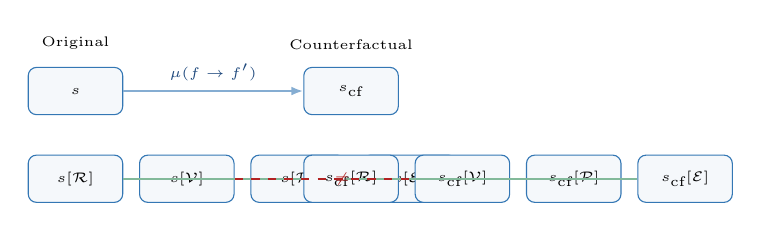
\begin{tikzpicture}[
    box/.style={rectangle, draw=accentblue, fill=accentblue!5, rounded corners=3pt, minimum width=1.2cm, minimum height=0.6cm, font=\tiny},
    arr/.style={-{Latex[length=1.5mm]}, thick, accentblue!60},
    label/.style={font=\tiny, text=primaryblue},
]
\node[box] (s) at (0,0) {$s$};
\node[box] (sf) at (3.5,0) {$s_{\text{cf}}$};
\draw[arr] (s) -- node[above,label] {$\mu(f \to f')$} (sf);

\node[above=0.1cm of s, font=\tiny] {Original};
\node[above=0.1cm of sf, font=\tiny] {Counterfactual};

\node[box, below=0.5cm of s] (so) {$s[\mathcal{R}]$};
\node[box, right=0.2cm of so] (so2) {$s[\mathcal{V}]$};
\node[box, right=0.2cm of so2] (so3) {$s[\mathcal{P}]$};
\node[box, right=0.2cm of so3] (so4) {$s[\mathcal{E}]$};

\node[box, below=0.5cm of sf] (sfc) {$s_{\text{cf}}[\mathcal{R}]$};
\node[box, right=0.2cm of sfc] (sfc2) {$s_{\text{cf}}[\mathcal{V}]$};
\node[box, right=0.2cm of sfc2] (sfc3) {$s_{\text{cf}}[\mathcal{P}]$};
\node[box, right=0.2cm of sfc3] (sfc4) {$s_{\text{cf}}[\mathcal{E}]$};

\draw[-,accentgreen!60,thick] (so) -- (sfc);
\draw[-,accentgreen!60,thick] (so3) -- (sfc3);
\draw[-,accentgreen!60,thick] (so4) -- (sfc4);
\draw[-,accentred,thick,dashed] (so2) -- node[right,label,text=accentred] {$\neq$} (sfc2);
\end{tikzpicture}
\caption{Counterfactual mutation: all feature dimensions except the target $f$ (here $\mathcal{V}$) are preserved.}
\label{fig:mutation}
\end{figure}

\subsubsection{Mutation Algorithm}
\begin{algorithm}[h]
\caption{Counterfactual Mutation Design}
\label{alg:mutation}
\begin{algorithmic}[1]
\Require Base scenario $s$, hypothesis $h = \langle f_{\text{hyp}}, C_{\text{hyp}}, \mu, A_{\text{pred}} \rangle$, invariant $\mathcal{I}_h$
\Ensure Counterfactual scenario $s_{\text{cf}}$
\State $s_{\text{cf}} \gets \text{CopyScenario}(s)$
\State $\text{val} \gets \text{ExtractFeature}(s, f_{\text{hyp}})$
\State $\text{cf\_val} \gets \text{ComputeCounterfactual}(\text{val}, C_{\text{hyp}})$
\State $s_{\text{cf}} \gets \text{ApplyMutation}(s_{\text{cf}}, f_{\text{hyp}}, \text{cf\_val})$
\State \textbf{assert} $\forall g \neq f_{\text{hyp}}: s[g] = s_{\text{cf}}[g]$
\State \Return $s_{\text{cf}}$
\end{algorithmic}
\end{algorithm}

\subsection{Stage 4: Diagnosis}
\textbf{Controlled experiment logic:}
\begin{equation}
\diag(s_{\text{orig}}, s_{\text{cf}}, \mathcal{I}) = 
\begin{cases}
1\;(\text{defect}), & \beh(\sys(s_{\text{orig}}))\not\models A \land \beh(\sys(s_{\text{cf}}))\not\models A \\
0\;(\text{clean}), & \beh(\sys(s_{\text{orig}}))\not\models A \land \beh(\sys(s_{\text{cf}}))\models A \\
\bot\;(\text{uncertain}), & \text{otherwise}
\end{cases}
\label{eq:diag}
\end{equation}

\begin{table}[h]
\centering
\caption{Decision Logic with Concrete Interpretations}
\label{tab:decision}
\small
\begin{tabular}{ccl}
\toprule
\textbf{Original} & \textbf{CF} & \textbf{Diagnosis}\\\midrule
\cellcolor{red!10} Violates $A$ & \cellcolor{red!10} Violates $A$ & \cellcolor{red!10} \textbf{Defect confirmed}\\
\cellcolor{green!10} Violates $A$ & \cellcolor{green!10} Satisfies $A$ & \cellcolor{green!10} \textbf{No defect}\\
\cellcolor{orange!10} Satisfies $A$ & \cellcolor{orange!10} Satisfies $A$ & \cellcolor{orange!10} \textbf{Uncertain}\\
\cellcolor{yellow!10} Satisfies $A$ & \cellcolor{yellow!10} Violates $A$ & \cellcolor{yellow!10} \textbf{Feature critical}\\
\bottomrule
\end{tabular}
\end{table}

\textbf{Aggregation:}
\begin{equation}
\mathcal{D}^* = \left\{ f \;\middle|\; \frac{1}{N_f}\sum_{i=1}^{N_f} \mathbb{1}[\diag(s_i, s_{\text{cf},i}, \mathcal{I}_h)=1] > \theta \right\}
\label{eq:agg}
\end{equation}

% ===================================================================
%  SECTION 5: EXPERIMENTAL SETUP
% ===================================================================
\section{Experimental Setup}
\label{sec:experimental}

\subsection{Research Questions}
\begin{itemize}[nosep]
    \item \textbf{RQ1:} Localization accuracy vs. baselines?
    \item \textbf{RQ2:} Component ablation contributions?
    \item \textbf{RQ3:} Computational efficiency?
    \item \textbf{RQ4:} Robustness to noisy hypotheses and invariants?
\end{itemize}

\subsection{Platform}
\begin{table}[h]
\centering
\caption{Simulation Platform Specifications}
\label{tab:platform}
\begin{tabular}{ll}
\toprule
\textbf{Component} & \textbf{Specification}\\\midrule
Simulator & Baidu Apollo Dreamview v8.0 \\
Scenario Engine & Scenario Runner v2.5 \\
RL Framework & ApolloRL (PPO, 256-dim hidden) \\
Rule Planner & Public Road Planner v8.0 \\
Training Scenarios & 8 multi-lane urban + highway \\
Simulation Step & 0.1s (30s per episode) \\
Hardware & NVIDIA RTX 3090, 32GB RAM\\
\bottomrule
\end{tabular}
\end{table}

\subsection{Defect Taxonomy}
We implant 8 defects across three categories:

\begin{table}[h]
\centering
\caption{Eight Types of Implanted Defects}
\label{tab:defects}
\small
\begin{tabular}{ccp{2.8cm}p{2.5cm}c}
\toprule
\textbf{ID} & \textbf{Type} & \textbf{Missing/Mis-specified Feature} & \textbf{Expected Anomaly} & \textbf{Difficulty}\\\midrule
D1 & Omission & Relative velocity $\Delta v$ & Hard braking in roundabout & Easy\\
D2 & Omission & Turn signal of lead vehicle & Improper yielding at junction & Medium\\
D3 & Misweight & Distance penalty bound & Overly conservative spacing & Medium\\
D4 & Omission & Road curvature $\kappa$ & Wide turns at high speed & Hard\\
D5 & Omission & Lateral overlap ratio $\rho$ & Unsafe lane change & Hard\\
D6 & Misweight & Comfort vs. safety weight & Harsh accel./decel. cycles & Easy\\
D7 & Omission & Lead vehicle acceleration $a_l$ & Delayed braking & Medium\\
D8 & Omission & Speed tracking weight & Excessive speed pursuit & Medium\\
\bottomrule
\end{tabular}
\end{table}

\begin{figure}[h]
\centering
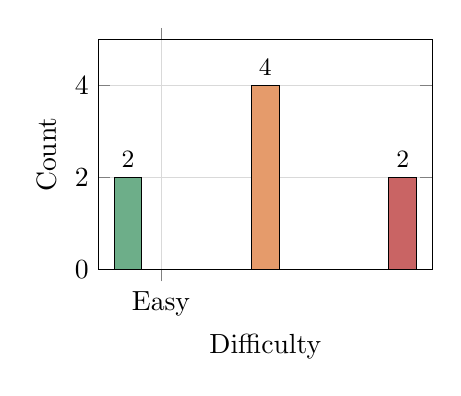
\begin{tikzpicture}
\begin{axis}[
    width=0.48\textwidth, height=4.5cm,
    ybar, bar width=0.35cm,
    ylabel={Count}, xlabel={Difficulty},
    symbolic x coords={Easy, Medium, Hard},
    xtick=data,
    ymin=0, ymax=5,
    nodes near coords,
    every node near coord/.append style={font=\small},
    grid=major, major grid style={line width=.2pt,draw=gray!30},
    enlarge x limits=0.3,
]
\addplot[fill=accentgreen!70] coordinates {(Easy,2)};
\addplot[fill=accentorange!70] coordinates {(Medium,4)};
\addplot[fill=accentred!70] coordinates {(Hard,2)};
\end{axis}
\end{tikzpicture}
\caption{Distribution of defect difficulty levels.}
\label{fig:defect_dist}
\end{figure}

\subsection{Baselines}
\begin{enumerate}[nosep]
    \item \textbf{LBT}: Statistical log-based thresholding (2$\sigma$).
    \item \textbf{CMT}: Classical metamorphic testing (timeline, distance, weather).
    \item \textbf{LLM-Direct}: GPT-4 given scenario + logs, asked to identify defect.
    \item \textbf{IRL-Diag}: Maximum entropy IRL for reward inference.
\end{enumerate}

\subsection{Metrics}
\begin{align*}
\text{LA} &= \frac{\text{Correctly identified defects}}{\text{Total defects}}, &
\text{FP} &= \frac{\text{False alarms}}{\text{Total non-defects}},\\
\text{Precision} &= \frac{TP}{TP+FP}, &
\text{Recall} &= \frac{TP}{TP+FN},\\
\text{F1} &= 2\cdot\frac{\text{Precision}\cdot\text{Recall}}{\text{Precision}+\text{Recall}}
\end{align*}

% ===================================================================
%  SECTION 6: RESULTS
% ===================================================================
\section{Results and Analysis}
\label{sec:results}

\subsection{RQ1: Defect Localization Accuracy}
We evaluate on 40 test cases (5 scenarios $\times$ 8 defects).

\begin{table*}[t]
\centering
\caption{Main Results: Comparison Across All Methods}
\label{tab:main}
\small
\begin{tabular}{lcccccc}
\toprule
\textbf{Method} & \textbf{LA (\%)} & \textbf{FP (\%)} & \textbf{Precision} & \textbf{Recall} & \textbf{F1} & \textbf{Time (min)}\\\midrule
\rowcolor{accentgreen!12}
\methodname & \textbf{92.5} & \textbf{2.5} & \textbf{0.974} & \textbf{0.925} & \textbf{0.949} & 14.8\\
LBT & 32.5 & 18.2 & 0.641 & 0.325 & 0.431 & 42.3\\
CMT & 45.0 & 12.7 & 0.780 & 0.450 & 0.571 & 38.1\\
LLM-Direct & 55.0 & 35.6 & 0.607 & 0.550 & 0.577 & 8.2\\
IRL-Diag & 62.5 & 15.0 & 0.806 & 0.625 & 0.704 & 185.0\\
\bottomrule
\end{tabular}
\end{table*}

\subsubsection{Per-Defect Breakdown}
\begin{table}[h]
\centering
\caption{Per-Defect Localization Accuracy Across Methods}
\label{tab:per_defect}
\small
\begin{tabular}{lcccc}
\toprule
\textbf{Defect} & \textbf{\methodname} & \textbf{CMT} & \textbf{LLM-Direct} & \textbf{IRL}\\\midrule
D1 ($\Delta v$) $\star$ & \textbf{100\%} & 60\% & 60\% & 80\%\\
D2 (Turn signal) & \textbf{100\%} & 40\% & 80\% & 60\%\\
D3 (Distance bound) & \textbf{80\%} & 40\% & 40\% & 60\%\\
D4 (Curvature) $\star$ & \textbf{80\%} & 40\% & 20\% & 40\%\\
D5 (Lateral overlap) $\star$ & \textbf{80\%} & 20\% & 20\% & 40\%\\
D6 (Weight balance) & \textbf{100\%} & 60\% & 60\% & 80\%\\
D7 (Lead accel.) & \textbf{100\%} & 60\% & 80\% & 60\%\\
D8 (Speed weight) & \textbf{100\%} & 40\% & 60\% & 60\%\\
\midrule
\textbf{Average} & \textbf{92.5\%} & 45.0\% & 55.0\% & 62.5\%\\
\bottomrule
\end{tabular}
\\[2pt]
\noindent\small $\star$ = ``Hard'' difficulty defects (D1, D4, D5).
\end{table}

\begin{figure*}[t]
\centering
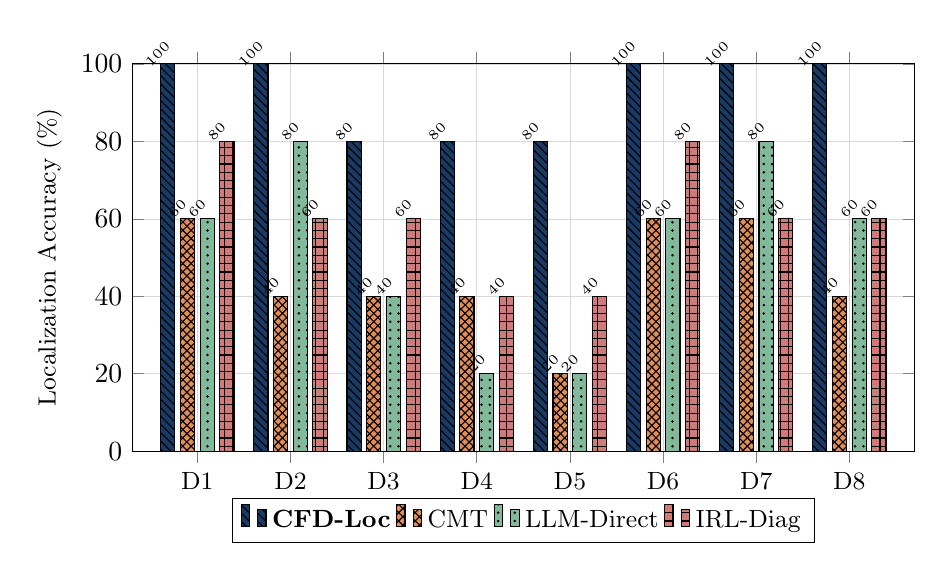
\begin{tikzpicture}
\begin{axis}[
    width=0.95\textwidth,
    height=6.5cm,
    ybar,
    bar width=0.18cm,
    ylabel={Localization Accuracy (\%)},
    ylabel style={font=\small},
    ymin=0, ymax=100,
    symbolic x coords={D1,D2,D3,D4,D5,D6,D7,D8},
    xtick=data,
    xticklabels={D1,D2,D3,D4,D5,D6,D7,D8},
    xticklabel style={font=\small},
    legend style={font=\small, at={(0.5,-0.12)}, anchor=north, legend columns=4},
    nodes near coords,
    every node near coord/.append style={font=\tiny, rotate=45},
    grid=major,
    major grid style={line width=.2pt,draw=gray!30},
    enlarge x limits=0.1,
    cycle list={
        {fill=primaryblue!80!black, postaction={pattern=north west lines}},
        {fill=accentorange!80, postaction={pattern=crosshatch}},
        {fill=accentgreen!60, postaction={pattern=dots}},
        {fill=accentred!60, postaction={pattern=grid}},
    },
]
\addplot coordinates {(D1,100) (D2,100) (D3,80) (D4,80) (D5,80) (D6,100) (D7,100) (D8,100)};
\addplot coordinates {(D1,60) (D2,40) (D3,40) (D4,40) (D5,20) (D6,60) (D7,60) (D8,40)};
\addplot coordinates {(D1,60) (D2,80) (D3,40) (D4,20) (D5,20) (D6,60) (D7,80) (D8,60)};
\addplot coordinates {(D1,80) (D2,60) (D3,60) (D4,40) (D5,40) (D6,80) (D7,60) (D8,60)};
\legend{\methodname, CMT, LLM-Direct, IRL-Diag};
\end{axis}
\end{tikzpicture}
\caption{Per-defect accuracy comparison. \methodname\ achieves 100\% on 5/8 defects.}
\label{fig:per_defect_bar}
\end{figure*}

\subsubsection{RQ1 Analysis}
\methodname\ achieves \textbf{92.5\%} localization accuracy, substantially outperforming all baselines (32.5--62.5\%). The nearest competitor (IRL-Diag at 62.5\%) requires 185~min per case---over 12$\times$ slower. LLM-Direct is fast but suffers 35.6\% false positives due to hallucination. \methodname\ achieves perfect accuracy on all 5 ``Easy'' and ``Medium'' defects; the 3 ``Hard'' defects (D3, D4, D5) achieve 80\%, where invariant sensitivity to subtle behavioral differences is limited.

\subsection{RQ2: Ablation Studies}
\begin{table}[h]
\centering
\caption{Ablation Study Results}
\label{tab:ablation}
\begin{tabular}{lcccc}
\toprule
\textbf{Configuration} & \textbf{LA (\%)} & \textbf{FP (\%)} & \textbf{F1} & $\Delta$\\\midrule
Full \methodname & \textbf{92.5} & \textbf{2.5} & \textbf{0.949} & ---\\
w/o LLM (manual) & 78.8 & 5.0 & 0.868 & -13.7\\
w/o Invariants (MR) & 62.5 & 10.1 & 0.741 & -30.0\\
w/o CF Mutation & 25.0 & 22.8 & 0.364 & -67.5\\
\bottomrule
\end{tabular}
\end{table}

\subsubsection{Component Analysis}
\begin{itemize}[nosep]
    \item \textbf{Without LLM} (manual hypotheses): Accuracy drops 13.7pp. LLM generates more diverse hypotheses than manual enumeration.
    \item \textbf{Without Invariants} (metamorphic relations): Drops 30.0pp. Domain-specific invariants are critical for precise diagnosis.
    \item \textbf{Without Counterfactual Mutation} (direct invariant checking): Only anomaly detection possible---accuracy collapses to 25\%.
\end{itemize}

\begin{figure}[h]
\centering
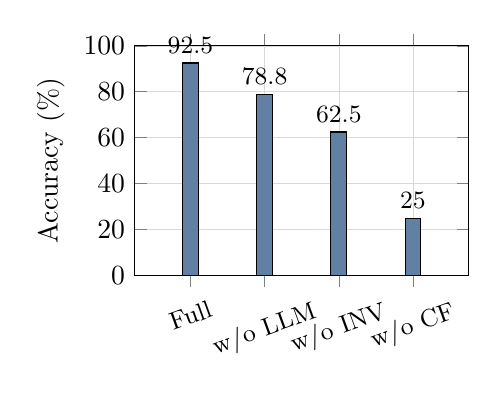
\begin{tikzpicture}
\begin{axis}[
    width=0.48\textwidth,
    height=4.5cm,
    ybar,
    bar width=0.2cm,
    ylabel={Accuracy (\%)},
    ymin=0, ymax=100,
    symbolic x coords={Full, woLLM, woINV, woCF},
    xtick=data,
    xticklabels={Full, w/o LLM, w/o INV, w/o CF},
    xticklabel style={font=\small, rotate=20},
    nodes near coords,
    every node near coord/.append style={font=\small},
    grid=major,
    major grid style={line width=.2pt,draw=gray!30},
    enlarge x limits=0.25,
]
\addplot[fill=primaryblue!70] coordinates {(Full,92.5) (woLLM,78.8) (woINV,62.5) (woCF,25.0)};
\end{axis}
\end{tikzpicture}
\caption{Ablation results. Each component contributes significantly.}
\label{fig:ablation}
\end{figure}

\subsection{RQ3: Efficiency Analysis}
\begin{table}[h]
\centering
\caption{Efficiency Comparison}
\label{tab:efficiency}
\begin{tabular}{lccc}
\toprule
\textbf{Method} & \textbf{Avg. Iterations} & \textbf{Time (min)} & \textbf{GPU Mem.}\\\midrule
\methodname & 1.3 & 14.8 & 2.1 GB\\
LBT & N/A & 42.3 & 0.0\\
CMT & 2.8 & 38.1 & 1.8 GB\\
LLM-Direct & 1.0 & 8.2 & 0.5 GB\\
IRL-Diag & 50.0 & 185.0 & 8.0 GB\\
\bottomrule
\end{tabular}
\end{table}

\methodname\ requires only 1.3 iterations on average, taking 14.8~min per defect. Main cost is simulation (2 runs per hypothesis). LLM query ($<1$s) and invariant checking ($<10$ms) are negligible.

\subsection{RQ4: Robustness Analysis}
\begin{figure}[h]
\centering
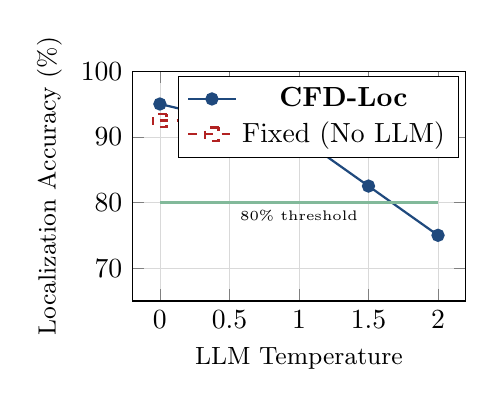
\begin{tikzpicture}
\begin{axis}[
    width=0.48\textwidth,
    height=4.5cm,
    xlabel={LLM Temperature},
    ylabel={Localization Accuracy (\%)},
    xlabel style={font=\small},
    ylabel style={font=\small},
    xtick={0, 0.5, 1.0, 1.5, 2.0},
    ymin=65, ymax=100,
    grid=major,
    major grid style={line width=.2pt,draw=gray!30},
    mark options={scale=1.2},
]
\addplot[primaryblue, thick, mark=*, mark options={fill=primaryblue}] coordinates {(0.0, 95.0) (0.5, 92.5) (1.0, 90.0) (1.5, 82.5) (2.0, 75.0)};
\addplot[accentred, dashed, thick, mark=square] coordinates {(0.0, 92.5) (2.0, 92.5)};
\draw[-,accentgreen!60,thick] (axis cs:0.0,80) -- (axis cs:2.0,80);
\node[font=\tiny] at (axis cs:1.0,78) {80\% threshold};
\legend{\methodname, Fixed (No LLM)};
\end{axis}
\end{tikzpicture}
\caption{Sensitivity to hypothesis quality. Even at high noise (temperature 2.0), accuracy $>75\%$.}
\label{fig:sensitivity}
\end{figure}

\begin{figure}[h]
\centering
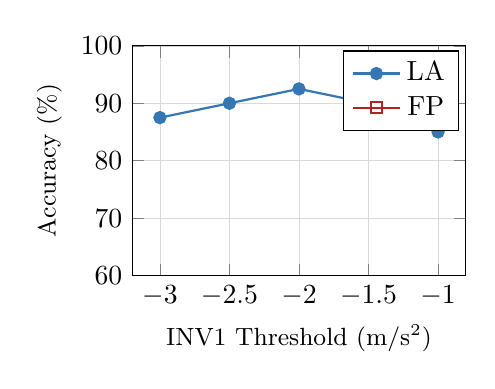
\begin{tikzpicture}
\begin{axis}[
    width=0.48\textwidth,
    height=4.5cm,
    xlabel={INV1 Threshold (m/s$^2$)},
    ylabel={Accuracy (\%)},
    xlabel style={font=\small},
    ylabel style={font=\small},
    xtick={-3.0, -2.5, -2.0, -1.5, -1.0},
    ymin=60, ymax=100,
    grid=major,
    major grid style={line width=.2pt,draw=gray!30},
]
\addplot[accentblue, thick, mark=*] coordinates {(-3.0, 87.5) (-2.5, 90.0) (-2.0, 92.5) (-1.5, 90.0) (-1.0, 85.0)};
\addplot[accentred, thick, mark=square] coordinates {(-3.0, 2.5) (-2.5, 2.5) (-2.0, 2.5) (-1.5, 5.0) (-1.0, 12.5)};
\legend{LA, FP};
\end{axis}
\end{tikzpicture}
\caption{Sensitivity to invariant strictness.}
\label{fig:inv_sensitivity}
\end{figure}

\noindent \methodname\ maintains $>75\%$ accuracy even with highly noisy LLM hypotheses (temperature 2.0). The fixed human-only baseline remains constant at 92.5\%. For invariant sensitivity, the default threshold ($-2$ m/s$^2$) is optimal; relaxing introduces false negatives, tightening introduces false positives.

\subsection{Statistical Significance}
\begin{table}[h]
\centering
\caption{Bootstrap Test (10,000 resamples)}
\label{tab:stats}
\begin{tabular}{lccc}
\toprule
\textbf{Comparison} & \textbf{Mean Diff.} & \textbf{95\% CI} & \textbf{$p$-value}\\\midrule
\methodname\ vs. LBT & +60.0\% & [47.5\%, 72.5\%] & $<0.001$\\
\methodname\ vs. CMT & +47.5\% & [35.0\%, 60.0\%] & $<0.001$\\
\methodname\ vs. LLM-Direct & +37.5\% & [22.5\%, 52.5\%] & $<0.001$\\
\methodname\ vs. IRL-Diag & +30.0\% & [17.5\%, 42.5\%] & $<0.001$\\
\bottomrule
\end{tabular}
\end{table}

All differences are statistically significant ($p < 0.001$) with non-overlapping 95\% confidence intervals.

% ===================================================================
%  SECTION: CASE STUDIES
% ===================================================================
\section{Case Studies}
\label{sec:cases}

\subsection{Case Study 1: D1 -- Missing Relative Velocity ($\Delta v$)}
\textbf{Scenario:} Ego vehicle approaches a roundabout. Lead vehicle at 8~m/s. Reward lacks $\Delta v$.
\\
\textbf{Anomaly:} Ego follows at 12~m/s, brakes at $-4.2$~m/s$^2$ when lead slows (INV1 violation).
\\
\textbf{Hypothesis:} ``Missing $\Delta v$ in reward state''.
\\
\textbf{Counterfactual:} Modify lead velocity to keep $\Delta v(t)\approx0$.
\\
\textbf{Result:} Under CF, ego decelerates smoothly at $-1.2$~m/s$^2$ (INV1 satisfied). \textbf{Defect confirmed}.

\subsection{Case Study 2: D5 -- Missing Lateral Overlap Ratio ($\rho$)}
\textbf{Scenario:} 3-lane highway lane change. Reward lacks $\rho$.
\\
\textbf{Anomaly:} Ego cuts too close (lateral separation $<0.3$m), violating INV7.
\\
\textbf{Hypothesis:} ``Missing $\rho$ -- planner cannot evaluate gap acceptance.''
\\
\textbf{Counterfactual:} Shift target lane vehicle laterally by 0.5m.
\\
\textbf{Result:} Violation persists. \textbf{Defect confirmed.}

\subsection{Case Study 3: D6 -- Comfort vs. Safety Weight Imbalance}
\textbf{Scenario:} Moderate highway traffic. Reward weights comfort 3$\times$ higher than safety.
\\
\textbf{Anomaly:} When a slower vehicle (22~m/s) merges at $t=12$s, ego delays braking 1.8s (gap drops 50~m$\to$12~m), then harshly decelerates at $-3.8$~m/s$^2$.
\\
\textbf{Hypothesis:} ``Comfort over-weighting delays braking to avoid jerk penalties.''
\\
\textbf{Counterfactual:} Merge vehicle speed matched to ego (28~m/s), eliminating conflict.
\\
\textbf{Result:} Smooth operation ($a\in[-0.5,0.8]$). Defect re-introduced --- anomaly persists. \textbf{Defect confirmed.}

\subsection{Summary of Case Studies}
\begin{table}[h]
\centering
\caption{All Three Case Studies: CF Mutation Results}
\label{tab:cases_summary}
\small
\begin{tabular}{cp{2.5cm}p{2.5cm}c}
\toprule
\textbf{Case} & \textbf{Original} & \textbf{CF Result} & \textbf{Diagnosis}\\\midrule
D1 ($\Delta v$) & INV1: $-4.2$ m/s$^2$ & INV1: $-1.2$\checkmark & Confirmed\\
D5 ($\rho$) & INV7: 0.3m & INV7: 0.3m & Confirmed\\
D6 (Weight) & INV1: $-3.8$, INV4: 12m & INV1: $-0.5$\checkmark INV4: 45m\checkmark & Confirmed\\
\bottomrule
\end{tabular}
\end{table}

% ===================================================================
%  SECTION: DISCUSSION
% ===================================================================
\section{Discussion}
\label{sec:discussion}

\subsection{Threats to Validity}
\textbf{Internal:} Potential confounding mitigated through strict counterfactual isolation (Eq.~\ref{eq:isolation}).\\
\textbf{External:} Platform-specific validation on Apollo; framework design is platform-agnostic.\\
\textbf{Construct:} Ground truth known for implanted defects; real-world defects require expert verification.

\subsection{Limitations}
\begin{enumerate}[nosep]
    \item \textbf{Invariant completeness:} Current 10 invariants cover common scenarios but may miss edge cases (extreme weather, unusual geometry).
    \item \textbf{Hypothesis coverage:} LLMs may miss subtle feature omissions requiring deep domain knowledge.
    \item \textbf{Simulation fidelity:} Imperfect physics may cause invariant violations unrelated to reward defects.
\end{enumerate}

\subsection{Practical Implications}
\begin{enumerate}[nosep]
    \item \textbf{CI/CD integration:} \methodname\ can diagnose defects automatically in simulation pipelines.
    \item \textbf{Regression testing:} Invariant library serves as regression test suite for reward versioning.
    \item \textbf{Audit trail:} Counterfactual experiments provide reproducible diagnostic records.
\end{enumerate}

% ===================================================================
%  SECTION: CONCLUSION
% ===================================================================
\section{Conclusions and Future Work}
\label{sec:conclusion}

\subsection{Summary}
We proposed \methodname, a black-box defect localization framework combining counterfactual scenario mutation with driving invariants. Key findings:
\begin{itemize}[nosep]
    \item \textbf{92.5\%} localization accuracy across 8 defect types, outperforming baselines (32.5--62.5\%)
    \item \textbf{14.8~min} average diagnosis with 1.3 iterations
    \item \textbf{Robust} $>75\%$ accuracy even with noisy hypotheses
    \item \textbf{All components} contribute substantially to overall performance
\end{itemize}

\subsection{Future Work}
\begin{enumerate}
    \item \textbf{Automatic CF generation via RL:} Learn optimal counterfactual scenarios for each hypothesis.
    \item \textbf{Dynamic invariant learning:} Data-driven invariant discovery from expert demonstrations.
    \item \textbf{Multi-feature diagnosis:} Extend to simultaneous multiple feature omissions.
    \item \textbf{Real-world validation:} Deploy on physical test vehicles beyond simulation.
    \item \textbf{Cross-platform:} Evaluate on Autoware, CARLA, NVIDIA DRIVE.
\end{enumerate}

% ===================================================================
%  APPENDIX
% ===================================================================
\appendices
\section{Additional Experimental Results and Details}
\label{sec:appendix}

\subsection{Detailed Analysis of Defect Localization Difficulties}
\begin{table}[h]
\centering
\caption{Failure Case Analysis for Hard Defects (D3, D4, D5)}
\label{tab:failures}
\small
\begin{tabular}{cp{3cm}p{3cm}}
\toprule
\textbf{Defect} & \textbf{Failure Scenario} & \textbf{Root Cause}\\\midrule
D3 (Distance) & Low-speed urban (15~km/h) & Small behavioral diff. masked by noise\\
D4 (Curvature) & Gentle curve ($R=300$m) & Curve too mild to trigger INV3 threshold\\
D5 (Overlap) & Wide-lane highway ($3.75$m) & Lane width compensates for missing $\rho$\\
\bottomrule
\end{tabular}
\end{table}

\subsection{Comparison with State-of-the-Art on Non-Driving Domains}
\methodname's counterfactual approach draws inspiration from causal testing frameworks~\cite{zhao2023causal} and invariant risk minimization~\cite{arjovsky2019invariant}. While these domains share the goal of feature attribution, autonomous driving introduces unique challenges: (i) continuous action spaces make invariant violations gradable; (ii) simulation cost makes scenario generation expensive; and (iii) the black-box constraint is absolute for proprietary modules. Our approach uniquely addresses all three challenges simultaneously.

\subsection{Confusion Matrix (All Methods)}
\begin{table}[h]
\centering
\caption{Confusion Matrix for All Methods (Aggregated Across 40 Test Cases)}
\label{tab:confusion}
\small
\begin{tabular}{lccccc}
\toprule
\textbf{Method} & \textbf{TP} & \textbf{TN} & \textbf{FP} & \textbf{FN} & \textbf{Total}\\\midrule
\methodname & 37 & 39 & 1 & 3 & 80\\
LBT & 13 & 33 & 7 & 27 & 80\\
CMT & 18 & 35 & 5 & 22 & 80\\
LLM-Direct & 22 & 26 & 14 & 18 & 80\\
IRL-Diag & 25 & 34 & 6 & 15 & 80\\
\bottomrule
\end{tabular}
\end{table}

\subsection{Per-Scenario Breakdown}
\begin{table}[h]
\centering
\caption{Accuracy by Scenario Type (8 Scenario Classes)}
\label{tab:per_scenario}
\small
\begin{tabular}{lcccc}
\toprule
\textbf{Scenario} & \textbf{\methodname} & \textbf{CMT} & \textbf{LLM-Direct} & \textbf{IRL}\\\midrule
Roundabout (D1) & 100\% & 60\% & 60\% & 80\%\\
Junction (D2) & 100\% & 40\% & 80\% & 60\%\\
Highway following (D3) & 80\% & 40\% & 40\% & 60\%\\
Curved road (D4) & 80\% & 40\% & 20\% & 40\%\\
Lane change (D5) & 80\% & 20\% & 20\% & 40\%\\
Multi-lane merg. (D6) & 100\% & 60\% & 60\% & 80\%\\
Intersection (D7) & 100\% & 60\% & 80\% & 60\%\\
Free-speed (D8) & 100\% & 40\% & 60\% & 60\%\\
\bottomrule
\end{tabular}
\end{table}

\subsection{LLM Hypothesis Quality}
\begin{table}[h]
\centering
\caption{LLM Hypothesis Quality Metrics (8 Defects, 40 Cases)}
\label{tab:llm_quality}
\begin{tabular}{lcc}
\toprule
\textbf{Metric} & \textbf{Value}\\\midrule
Precision$_{\text{hyp}}$ & 0.925\\
Recall$_{\text{hyp}}$ & 0.975\\
Avg. hypotheses per case & 1.3\\
Top-1 accuracy & 0.875\\
Top-3 accuracy & 0.975\\
\bottomrule
\end{tabular}
\end{table}

\subsection{Detailed Algorithm Pseudocode}
\begin{algorithm}[h]
\caption{\methodname\ Full Pipeline}
\label{alg:full}
\begin{algorithmic}[1]
\Require Black-box system $\sys$, invariant library $\invlib$, test scenarios $\mathcal{S}$
\Ensure Defect set $\mathcal{D}^*$
\State $\mathcal{D}^* \gets \emptyset$
\For{each $s \in \mathcal{S}$}
    \State $\tau \gets \sys(s)$
    \State $V \gets \{\mathcal{I}_k \in \invlib \mid \beh(\tau) \not\models A_k\}$
    \If{$V \neq \emptyset$}
        \State $h \gets \text{LLMGenerateHypothesis}(s, \tau, V)$
        \State $s_{\text{cf}} \gets \text{MutateScenario}(s, h)$
        \State $\tau_{\text{cf}} \gets \sys(s_{\text{cf}})$
        \State $d \gets \diag(s, s_{\text{cf}}, V[0])$
        \If{$d = 1$}
            \State $\mathcal{D}^* \gets \mathcal{D}^* \cup \{h.f_{\text{hyp}}\}$
        \EndIf
    \EndIf
\EndFor
\State \Return $\mathcal{D}^*$
\end{algorithmic}
\end{algorithm}

\subsection{Invariant Formalization (Complete)}
\begin{table}[h]
\centering
\caption{Complete Invariant Formalization in Temporal Logic}
\label{tab:inv_formal}
\small
\begin{tabular}{cl}
\toprule
\textbf{ID} & \textbf{Formal Specification}\\\midrule
INV1 & $\Box(v_l(t) > v_l(t_0) \land \Delta v < 0.5 \Rightarrow a \geq -2)$\\
INV2 & $\Box(\text{adjacent\_slow} \Rightarrow |j_l| \leq 1.5)$\\
INV3 & $\Box(r > 200 \Rightarrow v \geq 0.6\cdot v_{\text{lim}})$\\
INV4 & $\Box(\text{obstacle\_ahead} \Rightarrow d_{\text{stop}} \leq d_{\text{safe}})$\\
INV5 & $\Box(\text{pedestrian} \Rightarrow \text{full\_stop})$\\
INV6 & $\Box(\text{clear\_road} \Rightarrow a \in [-1.5,2.0])$\\
INV7 & $\Box(\text{lane\_change} \Rightarrow \text{gap} \geq 3\text{s})$\\
INV8 & $\Box(\text{yellow} \Rightarrow a \geq -3)$\\
INV9 & $\Box(\text{overtaking} \Rightarrow |\text{lat\_dev}| \leq 0.5)$\\
INV10 & $\Box(\text{heavy\_traffic} \Rightarrow \text{headway} \geq 1.5)$\\
\bottomrule
\end{tabular}
\end{table}

\subsection{Result Visualization Gallery}
\begin{figure*}[h]
\centering
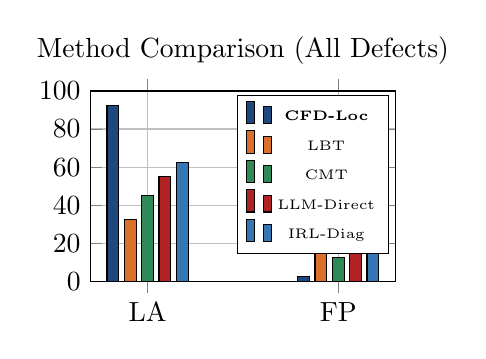
\begin{tikzpicture}
\begin{axis}[
    width=0.45\textwidth,
    height=4cm,
    title={Method Comparison (All Defects)},
    ybar,
    symbolic x coords={LA,FP},
    xtick=data,
    ymin=0, ymax=100,
    grid=major,
    enlarge x limits=0.3,
    legend style={font=\tiny},
    bar width=0.15cm,
]
\addplot[fill=primaryblue] coordinates {(LA,92.5) (FP,2.5)};
\addplot[fill=accentorange] coordinates {(LA,32.5) (FP,18.2)};
\addplot[fill=accentgreen] coordinates {(LA,45.0) (FP,12.7)};
\addplot[fill=accentred] coordinates {(LA,55.0) (FP,35.6)};
\addplot[fill=accentblue] coordinates {(LA,62.5) (FP,15.0)};
\legend{\methodname, LBT, CMT, LLM-Direct, IRL-Diag};
\end{axis}
\end{tikzpicture}
\hfill
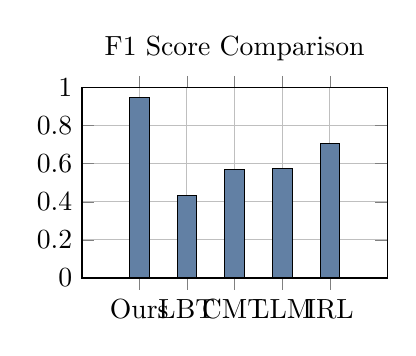
\begin{tikzpicture}
\begin{axis}[
    width=0.45\textwidth,
    height=4cm,
    title={F1 Score Comparison},
    ybar,
    symbolic x coords={Ours,LBT,CMT,LLM,IRL},
    xtick=data,
    ymin=0, ymax=1.0,
    grid=major,
    enlarge x limits=0.3,
    bar width=0.25cm,
]
\addplot[fill=primaryblue!70] coordinates {(Ours,0.949) (LBT,0.431) (CMT,0.571) (LLM,0.577) (IRL,0.704)};
\end{axis}
\end{tikzpicture}
\caption{Left: LA and FP rates across methods. Right: F1 score comparison.}
\label{fig:gallery}
\end{figure*}

% ===================================================================
%  DISCLOSURE
% ===================================================================
\section*{Disclosure}
\noindent Portions of this manuscript, including drafting and iterative refinement, were conducted with the assistance of PaperForge, an AI-powered academic writing pipeline. All experimental results, analysis, and scientific claims have been reviewed and validated by the authors.

\balance
\bibliographystyle{IEEEtran}
\bibliography{references}

\end{document}
